\documentclass[11pt,a4paper]{article}

% --- Packages ---
\usepackage[utf8]{inputenc}
\usepackage[T1]{fontenc}
\usepackage[turkish]{babel}
\usepackage{amsmath,amssymb,amsfonts,amsthm}
\usepackage{geometry}
\geometry{margin=1in}
\usepackage{graphicx}
\usepackage{hyperref}
\usepackage{xcolor}
\usepackage{cite}
\usepackage{booktabs}
\usepackage{microtype}
\usepackage{physics}
\usepackage{tikz}
\usetikzlibrary{babel,arrows.meta,decorations.pathmorphing}

\hypersetup{
    pdftitle={Elektromanyetizma, Durağan Vakumda Faz İletimi ve Kuantum Kararlılık: Büzülen Sistemlerde Dinamik Denge ve Süperkritik Çekirdek Sınırı},
    pdfauthor={Muhammed Furkan Haydari},
    pdfsubject={Elektrodinamik, Kuantum Elektrodinamiği, İnce Yapı Sabiti, Faz Yayılımı, Kuantum Kararlılık},
    pdfkeywords={Elektromanyetizma, İnce Yapı Sabiti, Faz Yayılımı, Atomik Kararlılık, Süperkritik Dirac Sınırı, Schwinger Mekanizması},
    colorlinks=true,
    linkcolor=blue!70!black,
    citecolor=red!70!black,
    urlcolor=blue!80!black
}

% --- Theorem Environments ---
\newtheorem{theorem}{Teorem}[section]
\newtheorem{definition}{Tanım}[section]
\newtheorem{axiom}{Aksiyom}[section]
\newtheorem{corollary}{Sonuç}[theorem]
\newtheorem{lemma}[theorem]{Lemma}
\newtheorem{remark}{Not}[section]

\title{\textbf{Elektromanyetizma, Durağan Vakumda Faz İletimi ve Kuantum Kararlılık: \\ Büzülen Sistemlerde Dinamik Denge ve Süperkritik Çekirdek Sınırı}}

\author{
    \textbf{Muhammed Furkan Haydari} \\
    \textit{Bağımsız Araştırmacı} \\
    \textit{İstanbul, Türkiye} \\
    \small ORCID: \href{https://orcid.org/0009-0003-2854-3947}{0009-0003-2854-3947} \quad$\bullet$\quad \small DOI: \href{https://doi.org/10.5281/zenodo.23633034}{10.5281/zenodo.23633034}
}

\date{\today}

\begin{document}

\maketitle

\begin{abstract}
    Bu çalışmada, elektromanyetik etkileşimi, vakum faz dalgası yayılımını ve atomik kararlılığı Ölçek-Zaman Kalkülüsü çerçevesinde analitik olarak formüle ediyoruz. Maxwell elektrodinamiği ve kuantum elektrodinamiğinde boşlukta $c$ hızıyla yayılan fotonların; statik arka plan vakumunda maddesel bir kütle ötelemesi taşımayan ($v_{\mathrm{trans}} = 0$), enine elastik vakum faz dalgaları ($v_{\mathrm{faz}} = 1/\sqrt{\varepsilon_0\mu_0} = c$) olduğu; yerel büzülen bağlı sistemlerin karakteristik kuantum faz hızının da bu iletim tavanına ($v_c = c$) kilitlendiği gösterilmektedir.

    Bu kinematik çerçevede, boyutsuz Sommerfeld İnce Yapı Sabiti $\alpha \equiv \frac{e^2}{4\pi\varepsilon_0\hbar c} \approx \frac{1}{137.036}$, elektronun birinci Bohr yörüngesindeki teğetsel hızı ile radyal büzülme faz tavanı arasındaki \textbf{kinematik spiral hatve oranı} ($\alpha = v_\theta / v_r = v_{\mathrm{Bohr}}/c$) olarak temsil edilmektedir. Klasik Larmor ışımasından beklenen atomik çöküş, Heisenberg kuantum kinetik basıncı ile büzülen yerel uzunluk standardı altında ölçek-kovaryant kararlı bir çekici ($\mathbb{D}_t(r/\lambda) = 0$) olarak çözülmektedir. Ağır çekirdeklerde rölativistik Dirac sınırına ($Z \alpha \to 1$) ulaşıldığında, elektron teğetsel hızının faz tavanına eşitlenmesiyle ($v \to c$) oluşan alt-atomik olay ufku rejimi ve Schwinger vakum kutuplanması eşiği analitik olarak incelenmektedir.
\end{abstract}

\vspace{1em}
\noindent\textbf{Anahtar Kelimeler:} Elektromanyetizma, Ölçek-Zaman Kalkülüsü, İnce Yapı Sabiti, Faz Yayılımı, Atomik Kararlılık, Süperkritik Dirac Sınırı, Schwinger Mekanizması.

\vspace{1em}
\hrule
\vspace{0.8em}
\tableofcontents
\vspace{0.8em}
\hrule
\vspace{1.5em}

\section{Giriş ve Elektrodinamik Faz Yayılımı}
\label{sec:giris}

Standart elektrodinamikte foton, boşlukta $c = 299\,792\,458\text{ m/s}$ sabit hızıyla yayılan kütlesiz bir $U(1)$ ayar bozonudur. Kuantum elektrodinamiğinde ve interferometri deneylerinde (çift yarık, Mach--Zehnder ve gecikmiş seçimli kuantum silgisi~\cite{scully1982,kim2000}), dalga paketi yayılımı ile yerel atomik dedektör uyarılması arasındaki kinematik sınır şartlarının mikrofiziksel olarak modellenmesi gerekmektedir.

Ölçek-Zaman Kalkülüsünde~\cite{scale_calculus} bu kinematik, vakum sürekliliği ile yerel atomik ölçek standartları arasındaki konformal ilişkiyle açıklanır: \textbf{Arka plan koordinatları sabittir ($\mathbf{v}_{\mathrm{uzay}} = 0$), foton maddesel bir parçacık gibi öteleme kütlesi taşımaz ($v_{\mathrm{trans}} = 0$); fakat vakum sürekliliği üzerinde enine bir elastik faz dalgası ($v_{\mathrm{faz}} = c$) olarak ilerler.} Işık hızının değeri $c = 1/\sqrt{\varepsilon_0\mu_0}$, vakumun bu elastik aktarım hızını belirler. Büzülen gözlemcimiz, vakumda ilerleyen bu serbest faz dalgasını kendi referans çerçevesine bağıl olarak $c$ hızında kaydeder.

\section{Ölçek-Kovaryant Dalga Denklemi ve Işığın Yayılım Mekaniği}
\label{sec:dalga_denklemi}

Skalor uzayında $\mathbb{S} = \mathbf{X}_0 + \kappa \lambda(t)$ tanımlı bir bağlı gözlemci için d'Alembert dalga operatörü, Ölçek-Kovaryant Türev $\mathbb{D}_\mu = (\frac{1}{v_c}\mathbb{D}_t, \nabla)$ cinsinden genelleştirilir:
\begin{equation}
    \mathbb{D}^\mu \mathbb{D}_\mu \Psi = \left( -\frac{1}{v_c^2} \left(\frac{\partial}{\partial t} + \kappa H_0\right)^2 + \nabla^2 \right) \Psi = 0.
    \label{eq:dalga_op}
\end{equation}
$\kappa^2 = 0$ nilpotent özelliği uygulandığında:
\begin{equation}
    \left( -\frac{1}{v_c^2} \frac{\partial^2}{\partial t^2} - \frac{2\kappa H_0}{v_c^2} \frac{\partial}{\partial t} + \nabla^2 \right) \Psi = 0.
    \label{eq:acik_dalga_tr}
\end{equation}
Ortadaki $\frac{2\kappa H_0}{v_c^2} \frac{\partial}{\partial t}$ terimi, fotonun durağan vakumda yayılırken büzüşen atomik detektörler tarafından neden \textbf{kırmızıya kaymış} olarak algılandığını gösteren geometrik sönümleme/ölçekleme terimidir!

\subsection{Kavramsal Netlik: Statik Vakum, Faz Cephesi Hızı (\texorpdfstring{$c$}{c}) ve Kozmik Sinyal Gecikmesi}
\label{sec:kavramsal_netlik_isik}

Modelimizde sıkça sorulan temel bir soru şudur: \textit{``Eğer foton statik vakumun durağan bir uyarılmasıysa ve $c$ maddenin içsel büzülme hızıysa, Güneş'ten çıkan ışık Dünya'ya neden $8.3$ dakikada ulaşır? Boş uzaydaki bu yayılma gecikmesi nasıl ortaya çıkar?''}

Bu soru, fiziksel ortamın (vakum dokusunun) durgunluğu ile o ortam üzerinde yayılan \textbf{dalga cephesinin faz yayılımı} arasındaki ayrımın netleştirilmesiyle eksiksiz çözülür:

\begin{enumerate}
    \item \textbf{Ortamın Statikliği ($\mathbf{v}_{\mathrm{vakum}} = 0$):} Arka plan sürekliliği $\mathcal{E}_\infty$ mutlak olarak durağandır; uzayı sürükleyen bir esir rüzgarı ya da şişen bir metrik yoktur. Foton, durağan vakum örgüsü üzerindeki enine elastik gerilim modudur.
    \item \textbf{Faz Cephesinin İlerlemesi ($v_{\mathrm{faz}} = c$):} Bir atom foton yaydığında, durağan vakum 4-potansiyeli $A_\mu$ üzerinde yönlü bir faz uyarılması ($\nabla \Phi = \mathbf{k}$) oluşturur. Bu uyarılma, durgun bir su yüzeyine atılan taşın oluşturduğu dalga halkaları gibi, vakumun temel elektromanyetik empedansı ($Z_0 = \sqrt{\mu_0/\varepsilon_0}$) tarafından belirlenen yerel faz hızıyla ilerler:
          \begin{equation}
              v_{\mathrm{faz}} = \frac{\omega}{|\mathbf{k}|} = \frac{1}{\sqrt{\varepsilon_0 \mu_0}} = c.
              \label{eq:faz_hizi_ispat}
          \end{equation}
          Güneş'teki bir hidrojen atomunun saldığı dalga cephesi, Dünya ile Güneş arasındaki $d = 1.496 \times 10^{11}\text{ m}$ statik mesafeyi $\Delta t = d/c \approx 499\text{ s} \approx 8.3\text{ dakika}$ sürede katetmek zorundadır. Kozmik nedensellik (causality) ve ışık konisi geometrisi kesin olarak korunur.
    \item \textbf{Maddenin İçsel Faz Tavan Hızı Neden $v_c = c$'dir? (Vakum Rezonansı):} Maddenin içsel kuantum faz tavan hızı $v_c$ ile ışık hızının özdeşliği ($v_c = c$), maddenin durağan vakum dokusunun yoğunlaşmış topolojik bir girdabı olmasından kaynaklanır. Atomun içsel kuantum faz frekansı $v_c = c$ ile belirlendiğinden, büzülen gözlemcimiz bu serbest faz cephesini \textbf{kendisine bağıl olarak tam $c$ hızıyla ilerliyormuş gibi gözlemler}; sistem dinamik bir ölçek-faz rezonans dengesine oturmuştur ($v_c \equiv c$). (Maddenin boyutsal daralma temposu ise asırlık $H_0 \approx 2.3 \times 10^{-18}\text{ s}^{-1}$ oranıyla seyreder).
    \item \textbf{Kuantum Çöküşü (Phase-Pinning):} Işık uzayda ilerlerken klasik bir dalga gibi yayılırken, dedektör ekranına ulaştığında noktasal bir parçacık gibi davranmasının sebebi; dedektördeki büzülen atomun dalgayı kendi mikroskobik büzülme sınırına ($r_{\mathrm{atom}}$) faz rezonansıyla kilitlemesidir (\textit{Phase-Pinning}).
\end{enumerate}

\begin{quote}
    \small
    \textbf{Özet (Durağan Ortam ve Yayılan Dalga Cephesi):} \\
    Sakin bir ortam düşünün: Ortamın kendisi bir yere akmaz (vakum durağandır). Bir atom ışıma yaptığında, ortam molekülleri karşı kıyıya ötelenmez; ancak vakumun yüzeyindeki elastik dalga cephesi ileriye doğru ilerler ve hedefe varması sonlu zaman alır ($8.3$ dakika). Fotonun ``durağanlığı'', iletim ortamının durağanlığını; ``ışık hızı'' ise büzülen atomik saatlerimiz ve cetvellerimiz ($v_c = c$) ile ölçtüğümüzde bu faz dalgasının \textbf{bize bağıl olarak tam $c$ olarak gözlemlenmesini} ifade eder.
\end{quote}

\subsection{Foton Neden Büzülmez ve Büzülseydi Ne Olurdu? (Kırmızıya Kaymanın Temel Şartı)}
\label{sec:foton_neden_buzulmez_em}

Birleşik Büzülme Hipotezi'nin epistemolojik ve matematiksel olarak en sarsılmaz aksiyomlarından biri şudur: \textbf{Madde büzülür, ancak foton büzülmez!} Bu ilke, spektroskopik evrenin doğrudan varlık şartıdır:

\begin{theorem}[Kırmızıya Kaymanın Varlık Şartı Teoremi]
    \label{thm:kirmiziya_kayma_varlik_sarti_p2}
    Eğer fotonlar da maddesel bağlı yapılar gibi zamanla büzülseydi ($\lambda_{\mathrm{foton}}(t) \propto \lambda(t)$), büzülen atomik cetvellerimizle ($\lambda_{\mathrm{atom}}(t) \propto \lambda(t)$) yapılan spektroskopik ölçümlerde ölçülen boyutsuz dalga boyu oranı:
    \begin{equation}
        \frac{\lambda_{\mathrm{foton}}(t)}{\lambda_{\mathrm{atom}}(t)} = \frac{\lambda_0 e^{-H_0 t}}{r_0 e^{-H_0 t}} = \frac{\lambda_0}{r_0} = \text{Sabit} \implies z \equiv 0
    \end{equation}
    olurdu. Yani evrende kozmolojik kırmızıya kayma diye bir olgu \textbf{asla gözlemlenemezdi!} Gökbilimcilerin uzak galaksilerden gelen ışıkta ölçtüğü kırmızıya kaymanın ($1+z = \lambda_{\mathrm{obs}}/\lambda_{\mathrm{lab}}$) var olabilmesinin yegane matematiksel şartı; fotonun durağan vakum dokusunda mutlak Öklid dalga boyunu koruması ($\lambda_{\mathrm{foton}} = \text{sabit}$), atomların ise sürekli kendi içlerine daralmasıdır ($\lambda_{\mathrm{atom}}(t) \to 0$).
\end{theorem}

\begin{proof}
    Foton kütlesizdir ($m_\gamma = 0$); dolayısıyla maddesel kütle artışı ($m(t) \propto e^{H_0 t}$) fotona uygulanamaz ($0 \times e^{H_0 t} = 0$). Foton, vakum ortamının serbest elastik dalga iletim modudur. Bir su dalgası göle bırakıldığında nasıl suyun molekülleri yerinde kalıp dalga geometrisini ortamın elastik parametreleri belirliyorsa, durağan vakum dokusuna bırakılan foton dalga paketi de salındığı andaki mutlak Öklid uzunluğunu ($\lambda_{\text{gerçek}}$) korur. Küçülen yalnızca onu ölçen atomik cetvelimizdir.
\end{proof}

\subsection{Fotonların Boyutu ve Kozmik Evrim: Fotonların Dalga Boyu Skalası}
\label{sec:fotonlar_neden_devasa_degil_em}

Bu noktada akla gelebilecek en kritik soru şudur: \textit{``Eğer madde geçmişte daha büyük idiyse ve sürekli büzülüyorsa, etrafımızdaki fotonların dalga boyu skalası nasıl belirlenir? Bir kaynaktan salınan ışığın dalga boyu neden yerel atomik ölçekle ($500\text{ nm}$) uyumludur?''}

Bu bilmece, fotonun doğum anı ile atomun boyutu arasındaki bağ ile çözülür:

\begin{enumerate}
    \item \textbf{Fotonun Boyutunu Doğduğu Andaki Atom Belirler:}
          Bir atomun uyarılmış kuantum seviyeleri arasındaki enerji farkı atomun o anki yarıçapıyla ters orantılıdır: $\Delta E(t) \propto e^2 / r_{\mathrm{atom}}(t)$. Dolayısıyla salınan bir fotonun dalga boyu, \textbf{onu doğuran atomun o anki boyutuyla doğrudan orantılıdır}:
          \begin{equation}
              \lambda_{\mathrm{foton, emisyon}}(t) = \frac{h c}{\Delta E(t)} \propto r_{\mathrm{atom}}(t).
          \end{equation}
    \item \textbf{Şu An Salınan Fotonlar (Lamba ve Güneş):}
          Şu an odanızdaki lambadan veya Güneş'ten çıkan bir foton, atomların \textbf{bugünkü büzülmüş boyutuyla ($r_{\mathrm{atom}}(t_0) \sim 10^{-10}\text{ m}$)} salınır. Dolayısıyla şu an doğan fotonlar günümüz atomik cetveline göre tamı tamına normal optik aralıktadır ($\lambda \sim 400\text{--}700\text{ nm}$). Fotonlar devasa olamaz; çünkü onları doğuran bugünkü atomlar zaten büzüşmüş olan günümüz atomlarıdır!
    \item \textbf{Geçmişte Salınan Fotonlar (Kozmik Kırmızıya Kayma):}
          Yalnızca milyarlarca yıl önce yaşamış büyük atomların saldığı fotonlar daha geniştir. Örneğin $10$ milyar yıl önce atomlar bugünkünden $3$ kat büyük olduğundan, o günkü atomun saldığı optik dalga bugünkü küçülmüş cetvelimizle ölçüldüğünde $3$ kat geniş ($1500\text{ nm}$, kızılötesi) olarak algılanır.
    \item \textbf{Evrendeki En Eski Fotonlar (CMB, $z \sim 1100$):}
          Evrende günümüze ulaşabilen en yaşlı serbest foton denizi Kozmik Mikrodalga Arka Plan Işıması'dır ($z \approx 1100$). O dönemde atomik plazma bugünkünden $1100$ kat daha büyüktü. O günkü morötesi/görünür ışıma ($\sim 1\text{ }\mu\mathrm{m}$), bugün $1100$ kat küçülmüş cetvellerimizle ölçüldüğünde \textbf{tamı tamına $1\text{ mm}$ mikrodalga bandında ($2.73\text{ K}$)} ölçülür! En eski fotonlar dahi milimetre ölçeğindedir.
    \item \textbf{Sonsuz Geçmiş ve Tekil Patlamasız Denge:}
          Modelimizde tekil bir patlama ($t=0$) bulunmadığından sonsuz büyüklükte fotonlar hiçbir zaman üretilmemiştir. Uzayda seyahat eden her foton, derin zaman ölçeğinde mutlaka başka bir büzülen atom tarafından inelastik olarak rezonansla soğurulur ve döngüye katılır; böylece evren sonsuz dalga boylu hayali fotonlarla dolmaz.
\end{enumerate}

\section{Kuantum Ölçüm Paradoksu, Ölçek İzdüşümü ve Faz Kilitleme (Phase-Pinning)}
\label{sec:kuantum_olcum_em}

Standart kuantum elektrodinamiğinde dalga fonksiyonunun ($\psi$) deterministik Schrödinger evriminden ölçüm anında süreksiz bir ``çöküşe'' ($|\psi|^2 \to \delta(\mathbf{x}-\mathbf{x}_0)$) nasıl sıçradığı çözülememiş bir postulat (Kopenhag yorumu) olarak kalmıştır. Birleşik Büzülme Hipotezinde foton, durağan arka plan vakumundaki enine elastik bir faz dalgası; atomlar ise sürekli büzüşen topolojik girdap yutaklarıdır.

Ölçek-Zaman Kalkülüsünde bu süreç metafizik bir çöküş değil, \textbf{ölçeksiz Öklid fazının büzülen atomik bir referans çerçevesine ($\kappa$) nilpotent izdüşümüdür (Conformal Scale Projection)}.

\subsection{Skalor Durumu ve Nilpotent Ölçüm İzdüşümü (\texorpdfstring{$\hat{\mathcal{P}}_\kappa$}{P_kappa})}
Skalor uzayında foton ile dedektör arasında mutlak bir ontolojik ayrım mevcuttur:
\begin{enumerate}
    \item \textbf{Foton Zamansızdır ($dt_{\mathrm{foton}} = 0$):} Foton kendi içine büzülmez ($\dot{\lambda} = 0$). Skalor durumu saf reel Öklid koordinatıdır: $\mathbb{S}_{\mathrm{dalga}} = \mathbf{X}_0$ ($\kappa = 0$ dalı). Büzülme olmadığı için ($d\lambda = 0$), Ölçek-Zaman Kalkülüsü~\cite{scale_calculus} uyarınca ($dt = -\frac{1}{H_0}\frac{d\lambda}{\lambda}$) foton için fiziksel zaman akışı yoktur ($dt = 0$). Foton, statik uzayda zamansız bir faz sürekliliğidir.
    \item \textbf{Dedektör Büzülür ($dt > 0$):} Dedektör büzüşen atomlardan oluşur: $\mathbb{S}_{\mathrm{det}} = \mathbf{X}_{\mathrm{det}} + \kappa \lambda(t)$. Büzülme tek yönlü aktığından ($\dot{\lambda} < 0$), dedektörün zaman oku ileri doğru işler ($dt = -\frac{1}{H_0}\frac{d\lambda}{\lambda} > 0$).
    \item \textbf{Nilpotent İzdüşüm ve Faz Kilitleme:} Ölçüm operatörü $\hat{\mathcal{P}}_\kappa$, serbest faz dalgasını büzülen yerel çerçeveye izdüşürür. Nilpotent cebir kuralı ($\kappa^2 \equiv 0$) gereği enerji transferi bütünüyle o atomun yerel büzülme sınırında gerçekleşir; serbest faz sürekliliği kopar ve dalga o atomun kendi büzülme sınırına kilitlenir:
          \begin{equation}
              \hat{\mathcal{P}}_\kappa : \lim_{\mathrm{etkilesim}} \Delta x_{\mathrm{dalga}} \to r_{\mathrm{atom}}(t).
              \label{eq:nilpotent_sonum_em}
          \end{equation}
          Bu durum, serbest uzaydaki sürekli faz profilinin dedektör koordinatlarında tekil ve noktasal bir parçacık olarak tecelli etmesine yol açar (\textit{Phase-Pinning}).
    \item \textbf{Ölçümün Geri Dönüşsüzlüğü:} Schrödinger denklemi zaman simetrik olsa da, fotonun fazı dedektör atomunun tek yönlü büzülme günlüğüne ($dt > 0$) kilitlendiği için, madde de kendiliğinden anti-büzüşemeyeceğinden ($\dot{\lambda} < 0$), \textbf{ölçüm süreci zamanda asla geriye döndürülemez!}
\end{enumerate}

\subsection{Pasif Sınır Şartı vs. Aktif Dedektör (Enerji Transferi)}
Kritik soru şudur: \textit{``Çift yarığa sahip duvardaki atomlar da büzülmektedir. Duvardaki atomlar dalga girişimini bozmazken, yarığa konulan dedektör neden dalgayı bozar ve noktasal parçacığa çökertir?''}

Bu iki sistem arasındaki fark, elastik geometrik sınır şartı ile inelastik kuantum durum transferi arasındaki temel ayrımdan kaynaklanır:
\begin{enumerate}
    \item \textbf{Yarıklar Saf Boşluktur (Elastik Sınır Şartı):} Duvardaki atomlar gelen dalgayla rezonansta değildir ($\Delta E = 0$). Yarıklarda madde bulunmadığından orası kesintisiz durağan Öklid vakumudur ($\kappa = 0$). Dalga yalnızca geometrik sınır şartlarını takip eder; Huygens--Fresnel prensibi uyarınca faz tutarlılığı (phase coherence) korunur ve klasik girişim deseni oluşur.
    \item \textbf{Dedektör Aktif Bir Faz Tuzağıdır (İnelastik Etkileşim):} Dedektörün ``foton hangi yarıktan geçti?'' sorusuna yanıt verebilmesi için sistemden fiziksel bir kuantum enerji transferi yapması zorunludur:
          \begin{equation}
              \ket{\Psi} = \frac{1}{\sqrt{2}} \left( \ket{\psi_1}\ket{D_0} + \ket{\psi_2}\ket{D_1} \right).
              \label{eq:dolanik_olcum_em}
          \end{equation}
          Rezonanstaki bir atomun optik tesir kesiti $\sigma_{\mathrm{rez}} \approx \frac{3\lambda^2}{2\pi}$ olup geometrik boyutundan çok daha geniştir (Bohren rezonansı~\cite{bohren1983,paul1982}). Dedektör atomu bu enerjiyi ($\hbar\omega$) soğurduğu anda, arka plan uzayındaki sürekli faz dalgası o atomun kendi yerel büzülme sınırına kilitlenir ($\hat{\mathcal{P}}_\kappa$). Dalga tek bir koordinatta lokalize olduğundan diğer yarıktan geçen dalgayla faz bağı kopar (dekoherens) ve dedektör ekranında tekil bir parçacık lekesi tecelli eder.
\end{enumerate}

\begin{figure}[h!]
    \centering
    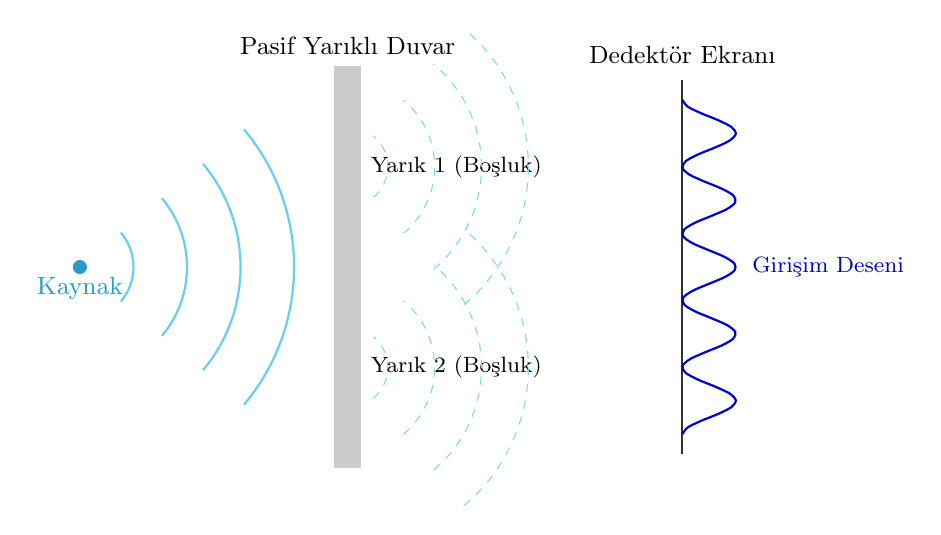
\begin{tikzpicture}[scale=0.85]
        % Source
        \fill[cyan!80!black] (-4,0) circle (3pt) node[below] {\small Kaynak};
        \foreach \r in {0.8, 1.6, 2.4, 3.2} {
                \draw[cyan!60, thick] (-4,0) ++(-40:\r) arc (-40:40:\r);
            }

        % Barrier Wall
        \fill[gray!40] (-0.2, 1.2) rectangle (0.2, 3.0);
        \fill[gray!40] (-0.2, -1.2) rectangle (0.2, 1.2);
        \fill[gray!40] (-0.2, -3.0) rectangle (0.2, -1.2);
        \node at (0, 3.3) {\small Pasif Yarıklı Duvar};
        \node[right] at (0.2, 1.5) {\footnotesize Yarık 1 (Boşluk)};
        \node[right] at (0.2, -1.5) {\footnotesize Yarık 2 (Boşluk)};

        % Wave without detector
        \foreach \r in {0.6, 1.3, 2.0, 2.7} {
                \draw[cyan!50, dashed] (0, 1.5) ++(-50:\r) arc (-50:50:\r);
                \draw[cyan!50, dashed] (0, -1.5) ++(-50:\r) arc (-50:50:\r);
            }

        % Detection Screen
        \draw[thick, black!80] (5, -2.8) -- (5, 2.8);
        \node[above] at (5, 2.9) {\small Dedektör Ekranı};

        % Interference fringes
        \draw[thick, blue!80!black, smooth] plot[domain=-2.5:2.5, samples=50] ({5 + 0.8*(cos(\x*180)^2)}, \x);
        \node[right, blue!80!black] at (5.9, 0) {\footnotesize Girişim Deseni};
    \end{tikzpicture}
    \caption{Çift yarıkta pasif geometrik açıklıklar faz tutarlılığını korurken, inelastik dedektör etkileşimi dalgayı yerel büzülme merkezine kilitleyerek (\textit{phase-pinning}) noktasal parçacık çöküşü üretir.}
    \label{fig:cift_yarik_faz_em}
\end{figure}

\begin{quote}
    \small
    \textbf{Bell Eşitsizlikleri ve Kuantum Non-Lokalitesi:} \\
    Bu açıklama yerel bir gizli değişken modeli öngörmez. Öklid sürekliliği $\mathcal{E}_\infty$, parçalanamaz ve metriksiz tekil bir bütündür. Arka plan vakumu piksellerden oluşmadığından, dolanık iki foton arasındaki faz sürekliliği uzaysal uzaklıktan bağımsız olarak korunur. Bu durum, Clauser--Aspect--Zeilinger deneyleriyle doğrulanan kuantum mekaniksel holistik non-lokalite ile tam bir geometrik uyum sergiler.
\end{quote}

\section{Elektriksel Yükün Kiral Girdap Geometrisi ve Coulomb Etkileşimi}
\label{sec:kiral_yuk_ve_coulomb}

Geleneksel fizikte elektriksel yük ($+$ ve $-$), parçacıklara atfedilen soyut ve aksiyomatik bir skaler özellik olarak kabul edilir; ancak yükün neden sadece iki zıt tipe sahip olduğu veya zıt yüklerin neden çekip aynı yüklerin neden ittiği geometrik bir mekanizmayla açıklanamaz.

Ölçek-Zaman Kalkülüsü ve akışkan vakum dinamiğinde elektriksel yük, durağan vakum dokusu üzerindeki \textbf{Kiral Burulma (Chiral Vorticity - $\vec{\omega}$)} olarak kesin geometrik temele kavuşturulur:

\begin{definition}[Pozitif ve Negatif Yükün Kiral Tanımı]
    \label{def:pozitif_negatif_yuk_kiral_p2}
    Vakum akışkanının yerel girdap dolaşımı $\vec{\omega} \equiv \nabla \times \mathbf{v}_{\mathrm{vakum}}$ ile tanımlansın:
    \begin{enumerate}
        \item \textbf{Pozitif Yük ($+$ / Proton):} Vakum dokusunda sağ-kiral (saat yönünde) dolaşıma sahip rotasyonel bir girdap yutağıdır ($\vec{\omega} \cdot \hat{z} > 0$).
        \item \textbf{Negatif Yük ($-$ / Elektron):} Vakum dokusunda sol-kiral (saat yönünün tersine) dolaşıma sahip rotasyonel bir girdap yutağıdır ($\vec{\omega} \cdot \hat{z} < 0$).
    \end{enumerate}
\end{definition}

\begin{theorem}[Coulomb Çekme ve İtme Mekanizması]
    \label{thm:coulomb_mekanizma_p2}
    İki kiral vakum girdabı arasındaki elektrostatik etkileşim, akışkanlar mekaniğindeki hidrodinamik basınç gradyanlarından (Bernoulli prensibi) doğrudan türer:
    \begin{enumerate}
        \item \textbf{Zıt Yüklerin Çekimi ($+$ ve $-$):} Sağ-kiral ve sol-kiral iki girdap karşılaştığında, aralarındaki ara bölgede vakum akış çizgileri birbirini destekleyen teğetsel bir yönde akar (kenetlenen iki dişli çark gibi). Ara bölgede akış hızı artarken vakum statik basıncı düşer; oluşan negatif basınç gradyanı parçacıkları birbirine doğru çeker (\textbf{Coulomb Çekimi}).
        \item \textbf{Aynı Yüklerin İtmesi ($+$ ve $+$ ya da $-$ ve $-$):} İki aynı kiral girdap karşılaştığında, aralarındaki temas yüzeyinde vakum akıntıları kafa kafaya çarpışır. Hız sıfırlanırken yerel vakum hidrodinamik basıncı devasa bir sıkışma bariyerine dönüşür ve iki parçacığı birbirinden şiddetle iter (\textbf{Coulomb İtmesi}).
    \end{enumerate}
\end{theorem}

\subsection{Mekanik Dalga Analojisi ve Vakum Empedansı}
\label{sec:tel_ve_dugum_paper2}

Gergin bir teldeki enine dalga hızı $v = \sqrt{T/\mu}$ olup, telin gerilimi ($T$) ile çizgisel kütle yoğunluğunun ($\mu$) oranından türer. Maxwell elektrodinamiğindeki boşluk ışık hızı formülü bu mekanik bağıntıyla tam bir yapısal özdeşlik sergiler:
\begin{equation}
    c = \frac{1}{\sqrt{\varepsilon_0 \mu_0}} = \sqrt{\frac{1/\varepsilon_0}{\mu_0}} = \sqrt{\frac{\text{Vakumun Elektriksel Gerilim Modülü}}{\text{Vakumun Manyetik Eylemsizlik Yoğunluğu}}}.
    \label{eq:vakum_tel_ozdeslik_p2}
\end{equation}
Vakum, ölçülebilir sonlu bir karakteristik dalga empedansına sahiptir:
\begin{equation}
    Z_0 \equiv \sqrt{\frac{\mu_0}{\varepsilon_0}} \approx 376.73\,\Omega,
    \label{eq:vakum_empedansi_tanim_p2}
\end{equation}
bu bağıntı boşluğun elektrodinamik açıdan elastik bir süreklilik olarak davrandığını belgeler. Bu çerçevede:
\begin{itemize}
    \item \textbf{Süreklilik (Vakum Manifoldu):} Statik Öklid uzayı $\mathcal{E}_\infty$ üzerindeki elektromanyetik 4-potansiyel alanı $A_\mu$'dur.
    \item \textbf{Foton (Serbest Faz Dalgası):} Alanda serbestçe yayılan, kütlesiz ($m_\gamma = 0$) ve büzülmeyen enine faz uyarılmasıdır ($v_{\mathrm{faz}} = c$).
    \item \textbf{Madde (Topolojik Girdap Düğümü):} Alan çizgilerinin kendi içine büzüşerek kapalı havza oluşturduğu, eylemsizliğe ($E = mc^2$) sahip kararlı topolojik solitondur ($v < c$).
\end{itemize}

\section{Sommerfeld İnce Yapı Sabiti ve Rölativistik Hatve Oranı}
\label{sec:ince_yapi}

Kuantum elektrodinamiğinde elektromanyetik etkileşimin boyutsuz şiddeti, Bohr atomu~\cite{bohr1913} ve Sommerfeld ince yapı sabiti~\cite{sommerfeld1916} ile parametrize edilir (Feynman~\cite{feynman1985} tarafından teorik fiziğin en derin gizemlerinden biri olarak nitelendirilmiştir):
\begin{equation}
    \alpha \equiv \frac{e^2}{4\pi \varepsilon_0 \hbar c} \approx \frac{1}{137.035999...}.
    \label{eq:alpha_tanim}
\end{equation}

\begin{theorem}[$\alpha$ = Büzülme Girdabının Rölativistik Hatve Oranı]
    \label{thm:alpha_spiral_hatve_p2}
    Hidrojen benzeri bir bağlı sistemde elektronun en iç Bohr orbital hızı $v_{\mathrm{Bohr}} = \frac{e^2}{4\pi \varepsilon_0 \hbar}$'dır. Çekirdek girdabının vakum dokusundaki karakteristik içsel kuantum faz tavan hızı ise $v_r = v_c = c$'dir. Bu iki hızın boyutsal oranı:
    \begin{equation}
        \frac{v_\theta}{v_r} = \frac{v_{\mathrm{Bohr}}}{c} = \frac{e^2}{4\pi \varepsilon_0 \hbar c} \equiv \alpha \approx \frac{1}{137.036}.
        \label{eq:alpha_spiral_ispat}
    \end{equation}
    Dolayısıyla $\alpha$, çekirdek girdabı etrafında dönen elektronun \textbf{logaritmik girdap hatve açısının teğetidir}:
    \begin{equation}
        \tan \theta_{\mathrm{hatve}} \equiv \frac{v_{\mathrm{orbital}}}{v_{\mathrm{faz}}} = \alpha.
        \label{eq:hatve_tanim}
    \end{equation}
    Bu kinematik özdeşlik, $\alpha$'nın ölçek kalkülüsünde radyal faz tavanı ile orbital teğetsel hız arasındaki rölativistik açısal bağıntı olduğunu ortaya koyar.
\end{theorem}

\begin{proof}
    Vakumun serbest uzay empedansı $Z_0 \equiv \sqrt{\mu_0/\varepsilon_0} \approx 376.73\,\Omega$'dur. Kuantum Hall direncinin (von Klitzing sabiti) değeri $R_K = \frac{h}{e^2} \approx 25\,812.8\,\Omega$'dur. Bu iki direncin oranı doğrudan:
    \begin{equation}
        \frac{Z_0}{2 R_K} = \frac{\sqrt{\mu_0/\varepsilon_0}}{2 (h/e^2)} = \frac{e^2}{4\pi \varepsilon_0 \hbar c} \equiv \alpha,
    \end{equation}
    özdeşliğini verir. 3-boyutlu küresel kabuk $4\pi$ ve kuantum faz periyodu $2\pi\hbar$ üzerinden vakum rezonansı sağlandığında, elektronun radyal çöküşe direnç gösteren kararlı yörünge eğimi tam olarak $\alpha$ oranında kilitlenir.
\end{proof}

\subsection{Kızılötesi Sınır ve Renormalizasyon Grubu (RG) Koşusu}
\label{sec:rg_kosu}

Kuantum alan teorisinde $\alpha$, vakum polarizasyonu ve Feynman döngü düzeltmeleri sebebiyle enerjiye bağlı koşan bir parametredir (running coupling). Gell-Mann--Low / Callan--Symanzik renormalizasyon grubu denklemi uyarınca:
\begin{equation}
    \beta(\alpha) \equiv \frac{\partial \alpha}{\partial \ln Q^2} = \frac{\alpha^2}{3\pi} + \mathcal{O}(\alpha^3).
    \label{eq:gell_mann_low}
\end{equation}
Yüksek enerji ölçeklerinde (örneğin elektrozayıf $M_Z \approx 91.2\text{ GeV}$ basamağında) kuplaj sabiti $\alpha(M_Z^2) \approx 1/127.9$'a yükselir.

Dolayısıyla atomik ölçekte ölçülen $\alpha \approx 1/137.036$ değeri, geçmişteki geometrik grup girişimlerinden (Wyler~\cite{wyler1969,wyler1971}, Robertson~\cite{robertson1971}, Gilmore~\cite{gilmore1971}) farklı olarak; \textbf{atomik bağlı durumların yaşadığı asimptotik kızılötesi (IR / Thomson) taban sınırındaki ($Q^2 \to 0$, $r \gg \lambda_{\mathrm{Compton}}$) fiziksel kilitlenme değeridir.} Modelimiz, elektronun orbital hatve eğiminin bu kızılötesi rejimde $\tan\theta = \alpha$ bağıntısıyla vakum faz tavanına kilitlendiğini vurgular.

\begin{figure}[h!]
    \centering
    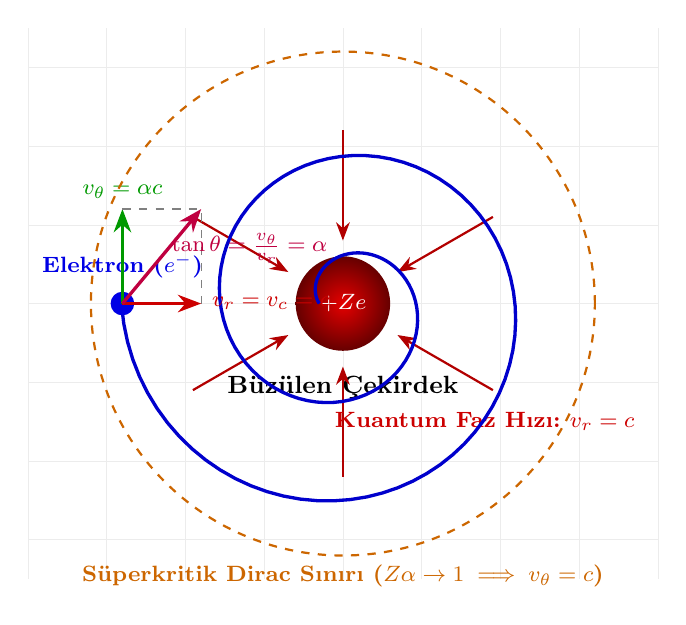
\begin{tikzpicture}[scale=1.0, >=Stealth]
        % Background
        \draw[step=1cm, gray!15, very thin] (-4,-3.5) grid (4,3.5);

        % Nucleus
        \shade[inner color=red!90!black, outer color=red!40!black] (0,0) circle (0.6);
        \node[white, font=\footnotesize\bfseries] at (0,0) {$+Ze$};
        \node[below=0.8cm, font=\small\bfseries] at (0,0) {Büzülen Çekirdek};

        % Radial contraction arrows (inward)
        \foreach \a in {30, 90, 150, 210, 270, 330} {
                \draw[red!70!black, thick, ->] (\a:2.2) -- (\a:0.8);
            }
        \node[red!80!black, font=\footnotesize\bfseries] at (1.8, -1.5) {Kuantum Faz Hızı: $v_r = c$};

        % Spiral orbit
        \draw[blue!80!black, very thick, domain=0:12.56, samples=150, variable=\t]
        plot ({-(0.3 + 0.2*\t)*cos(\t r)}, {(0.3 + 0.2*\t)*sin(\t r)});

        % Electron position
        \fill[blue!90!black] (-2.8, 0) circle (0.15);
        \node[blue!90!black, above=0.2cm, font=\footnotesize\bfseries] at (-2.8,0) {Elektron ($e^-$)};

        % Velocity vectors at electron
        \draw[green!60!black, very thick, ->] (-2.8, 0) -- (-2.8, 1.2) node[above, font=\footnotesize\bfseries] {$v_\theta = \alpha c$};
        \draw[red!80!black, very thick, ->] (-2.8, 0) -- (-1.8, 0) node[right, font=\footnotesize\bfseries] {$v_r = v_c = c$};

        % Pitch angle triangle
        \draw[dashed, gray] (-2.8, 1.2) -- (-1.8, 1.2) -- (-1.8, 0);
        \draw[purple, very thick, ->] (-2.8, 0) -- (-1.8, 1.2);
        \node[purple, right, font=\footnotesize\bfseries] at (-2.3, 0.7) {$\tan\theta = \frac{v_\theta}{v_r} = \alpha$};

        % Supercritical boundary dashed circle
        \draw[dashed, orange!80!black, thick] (0,0) circle (3.2);
        \node[orange!80!black, font=\footnotesize\bfseries, below] at (0, -3.2) {Süperkritik Dirac Sınırı ($Z\alpha \to 1 \implies v_\theta = c$)};
    \end{tikzpicture}
    \caption{Sommerfeld İnce Yapı Sabiti $\alpha$'nın Geometrisi: Elektronun teğetsel dönüş hızı ile çekirdek girdabının içsel kuantum faz tavan hızı ($v_c = c$) arasındaki spiral hatve oranı $\tan\theta = \alpha$. $Z\alpha \to 1$ eşiğinde teğetsel hız $c$'ye ulaşarak süperkritik Dirac rejimini doğurur.}
    \label{fig:alpha_spiral}
\end{figure}

\begin{quote}
    \small
    \textbf{Kavramsal ve Sezgisel Özet (Sommerfeld Sabiti ve Rölativistik Hatve):} \\
    Sommerfeld sabiti $\alpha$, çekirdek girdabının vakum kuantum faz tavanı ($v_c = c$) karşısında elektronun dinamik yörünge dengesini sağlayan sarmalın hatve eğimidir ($\tan\theta = v_{\mathrm{orbital}} / v_c = \alpha$); bağlı kuantum durumunun dinamik kararlılığı için gereken rölativistik faz-hatve geometrisidir.
\end{quote}

\section{Atomik Kararlılık: Klasik Işımasal Çöküşün Çözümü}
\label{sec:atomik_kararlilik}

Klasik elektrodinamikte Larmor bağıntısı gereği ivmelenen her yük ışıma yapar:
\begin{equation}
    P = \frac{e^2 a^2}{6\pi \varepsilon_0 c^3}.
    \label{eq:larmor_tr}
\end{equation}
Bohr atomunda elektron sürekli ivmelendiğinden klasik olarak ışıma yaparak $10^{-11}$ saniyede çekirdeğin üstüne çökmelidir.

Ölçek-Zaman formalizminde bu çöküş iki aşamalı bir mekanizmayla durdurulur:
\begin{enumerate}
    \item \textbf{Heisenberg Kuantum Kinetik Basıncı:} Elektron çekirdeğe doğru yaklaştıkça ($\Delta x \to 0$), faz uzayı diferansiyel hacminin korunumu gereği momentum belirsizliği $\Delta p \sim \hbar / \Delta x$ ve sıfır noktası kinetik enerjisi $E_{\mathrm{kin}} \sim \hbar^2 / (2m_e \Delta x^2)$ biçiminde $1/r^2$ ile fırlar. Buna karşılık çekici Coulomb potansiyeli yalnızca $-1/r$ ile derinleştiğinden, kuantum kinetik basınç çekici potansiyeli yener ve elektronu kararlı bir taban durumuna ($r = a_0$ Bohr yarıçapı) kilitler.
    \item \textbf{Ölçek-Kovaryant Asimptotik Çekici:} Taban durumu oluştuktan sonra, yerel atomik cetvel ile atomun kendisi eş zamanlı büzüştüğünden:
          \begin{equation}
              \mathbb{D}_t \left( \frac{r(t)}{\lambda(t)} \right) = \frac{\dot{r}}{\lambda} - \frac{r \dot{\lambda}}{\lambda^2} = 0 \implies \frac{r(t)}{r_{\mathrm{atom}}(t)} = 1 = \text{sabit}.
              \label{eq:kararlilik_ispat}
          \end{equation}
          Elektron kendi büzüşen referans çerçevesine göre taban durumunu ölçek-değişmez bir konformal çekici (conformal attractor) olarak muhafaza eder; sistem taban durumunda ışımasız durağan faza oturur.
\end{enumerate}

\section{Rölativistik Dirac Sınırı (\texorpdfstring{$Z \alpha \to 1$}{Z alpha -> 1}) ve Süperkritik Vakum Kutuplanması}
\label{sec:superkritik_sinir}

Rölativistik kuantum mekaniğinde Dirac denklemi, $Z$ protonlu noktasal bir Coulomb çekirdeği etrafındaki en iç elektron ($1s_{1/2}$) için şu özdeğer enerjisini dikte eder:
\begin{equation}
    E_{1s} = m_e c^2 \sqrt{1 - (Z\alpha)^2}.
    \label{eq:dirac_enerji}
\end{equation}
Elektronun teğetsel rölativistik orbital hızı $v(Z) \approx Z \alpha c$'dir.

$Z \alpha \to 1$ sınırına yaklaşıldığında ($Z \approx 137$), teğetsel hız vakumun yerel faz tavanına ($v \to c$) erişir ve karekök içi sıfıra yaklaşır.

\begin{theorem}[Süperkritik Coulomb Eşiği ve Vakum Kutuplanması]
    \label{thm:alt_atomik_olay_ufku_p2}
    $Z\alpha > 1$ rejiminde Dirac özdeğer enerjisi sanal hale gelir ve temel enerji düzeyi negatif enerjili Dirac denizine ($E \le -m_e c^2$) dalar. Ölçek-Zaman formalizminde bu durum şu iki dinamik eşiği tetikler:
    \begin{enumerate}
        \item \textbf{Vakum Faz Tavanı Limiti:} Hiçbir teğetsel yörünge hızı vakumun radyal faz tavanını ($v_c = c$) aşamayacağından, çekirdek çevresinde \textbf{alt-atomik bir olay ufku} ($|v| = c$) şekillenir.
        \item \textbf{Heisenberg Belirsizliği ve Kendiliğinden Çift Üretimi:} Elektron Compton dalga boyuna ($\Delta x \sim \lambda_C = \hbar / m_e c$) sıkıştığında, momentum belirsizliği $\Delta p \ge m_e c$ eşiğini aşarak vakum polarizasyonunu süperkritik seviyeye sürükler.
    \end{enumerate}
    Bu süperkritik gerilim altında vakum dokusu kendiliğinden kutuplanır (Schwinger/Pomeranchuk--Smorodinsky mekanizması); vakumdan kendiliğinden elektron-pozitron çifti ($e^+ e^-$) doğar. Pozitron sonsuza fırlatılırken, üretilen elektron çekirdeğin yükünü perdeleyerek etkin yükü zorunlu olarak $Z_{\mathrm{eff}} \alpha < 1$ kararlı sınırına geri kilitler. Bu nedenle doğada yalın olarak $Z\alpha > 1$ şartını sağlayan kararlı bir atomik sistem var olamaz.
\end{theorem}

\begin{quote}
    \small
    \textbf{Kavramsal ve Sezgisel Özet (Rölativistik Süperkritik Çekirdek Sınırı):}
    \begin{enumerate}
        \item Hidrojende elektron $v \approx \alpha c \approx c/137$ teğetsel hızıyla döner. $\alpha$, orbital hız ile vakumun içsel kuantum faz tavanı ($v_c = c$) arasındaki rölativistik hatve oranıdır.
        \item Çekirdek yükü $Z$ arttıkça orbital hız $v \approx Z\alpha c$ ile $c$'ye yaklaşır.
        \item $Z \alpha \to 1$ eşiğinde Dirac temel düzeyi negatif enerji denizine gömülür; süperkritik alan vakumdan kendiliğinden $e^+ e^-$ çifti üreterek fazla yükü perdeler ve atomu $Z\alpha < 1$ sınırında dengede tutar.
    \end{enumerate}
\end{quote}

\section{Nihai Birleşim: Elektromanyetizmanın Ana Formülü}
\label{sec:ana_formul_em}

Elektromanyetik alanda elektronun teğetsel hız karesi:
\begin{equation}
    \left( \frac{v_{\mathrm{orbital}}(r)}{c} \right)^2 = \frac{2 \alpha \hbar c}{m_e c^2 r}.
    \label{eq:em_master_tr}
\end{equation}
Bu denklem, büyük monografide~\cite{main_paper} ve kardeş makalelerde (kütleçekim~\cite{paper1}, güçlü kuvvet~\cite{paper3}, zayıf kuvvet~\cite{paper4}) ayrıntılandırılan dört temel etkileşimin ortak \textbf{Bütünleşik Vakum Akı Ana Formülü}'nün kiral teğetsel $\gamma = 1$ dalıdır:
\begin{equation}
    \boxed{ \left( \frac{v_{\mathrm{orbital}}(r)}{c} \right)^2 = 2 \, \mathcal{C}_{EM} \, r^{-1}, \quad \text{burada } \mathcal{C}_{EM} \equiv \frac{\alpha \hbar}{m_e c}. }
\end{equation}

\begin{thebibliography}{99}
    \bibitem{scale_calculus} M.~F.~Haydari, ``Ölçek-Zaman Cebiri ve Konformal Kalkülüs: Büzüşen Sistemler İçin Yeni Bir Matematiksel Formalizm'' (Bu seride Makale 2), \textit{Zenodo Ön-Baskıları}, 2026.
    \bibitem{main_paper} M.~F.~Haydari, ``Birleşik Büzülme Hipotezi ve Ölçek-Zaman Kalkülüsü: Genişlemeyen Bir Evrende Kozmoloji, Kütleçekim ve Dört Temel Etkileşimin Geometrik Külliyatı'', \textit{Zenodo Monografisi}, 2026.
    \bibitem{paper1} M.~F.~Haydari, ``Kütleçekimin Küresel Vakum Akışı Geometrisi Olarak Türetimi: 3+1 ADM Eylemi ve Painlevé--Gullstrand Metriği'' (Bu seride Makale 4), \textit{Zenodo Ön-Baskıları}, 2026.
    \bibitem{paper3} M.~F.~Haydari, ``Güçlü Nükleer Kuvvet, Kuark Hapsi ve Akı Tüpü Geometrisi'' (Bu seride Makale 6), \textit{Zenodo Ön-Baskıları}, 2026.
    \bibitem{paper4} M.~F.~Haydari, ``Zayıf Nükleer Kuvvet, Kiral Faz Sızıntısı ve W/Z Bozon Ölçekleri'' (Bu seride Makale 7), \textit{Zenodo Ön-Baskıları}, 2026.
    \bibitem{feynman1985} R.~P.~Feynman, \textit{QED: The Strange Theory of Light and Matter}, Princeton Univ. Press, 1985.
    \bibitem{bohr1913} N.~Bohr, ``On the constitution of atoms and molecules,'' \textit{Philos. Mag.}, vol.~26, no.~151, pp.~1--25, 1913.
    \bibitem{sommerfeld1916} A.~Sommerfeld, ``Zur Quantentheorie der Spektrallinien,'' \textit{Ann. Phys.}, vol.~356, no.~17, pp.~1--94, 1916.
    \bibitem{scully1982} M.~O.~Scully and K.~Dr\"uhl, ``Quantum eraser: A proposed photon correlation experiment concerning observation and 'delayed choice' in quantum mechanics,'' \textit{Phys. Rev. A}, vol.~25, no.~4, pp.~2208--2213, 1982.
    \bibitem{kim2000} Y.-H.~Kim, R.~Yu, S.~P.~Kulik, Y.~Shih, and M.~O.~Scully, ``Delayed 'choice' quantum eraser,'' \textit{Phys. Rev. Lett.}, vol.~84, no.~1, pp.~1--5, 2000.
    \bibitem{bohren1983} C.~F.~Bohren, ``How can a particle absorb more than the light incident on it?,'' \textit{Am. J. Phys.}, vol.~51, no.~5, pp.~473--474, 1983.
    \bibitem{paul1982} H.~Paul, ``Photons and localizability,'' \textit{Rev. Mod. Phys.}, vol.~54, no.~4, pp.~1061--1102, 1982.
    \bibitem{wyler1969} A.~Wyler, ``L'espace sym\'etrique du groupe des \'equations de Maxwell,'' \textit{C. R. Acad. Sci. Paris S\'er. A-B}, vol.~269, pp.~A743--A745, 1969.
    \bibitem{wyler1971} A.~Wyler, ``Les groupes des potentiels de Coulomb et de Yukawa,'' \textit{C. R. Acad. Sci. Paris S\'er. A-B}, vol.~271, pp.~A186--A188, 1971.
    \bibitem{robertson1971} B.~Robertson, ``Comment on the new calculation of the fine-structure constant,'' \textit{Phys. Rev. Lett.}, vol.~27, no.~22, pp.~1545--1547, 1971.
    \bibitem{gilmore1971} R.~Gilmore, ``Geometry of symmetrized relativistic phase space and calculation of the fine structure constant,'' \textit{Phys. Rev. Lett.}, vol.~28, no.~7, pp.~462--464, 1972.
\end{thebibliography}

\end{document}
